\chapter{Eigenvalue and Eigenvector}

\section{Basics}

\begin{definition}
    An \textbf{eigenvector}  of an \(n \times  n\)  matrix A is a nonzero vector x such that \(Ax = \lambda x\) for some scalar \(\lambda \). 
    A scalar \(\lambda \) is called an \textbf{eigenvalue}  of A if there is nontrivial solution x of \(Ax = \lambda x\) such an x is called an eigenvector corresponding to \(\lambda \)       
\end{definition}

\begin{remark}
    The eigenvector must be nonzero, but the eigenvalue can be 0.
\end{remark}

Considering the characteristic function \((A - \lambda I)x = 0\), due to the definition, we have an eigenvalue only if we have a nontrivial solution x (which is the eigenvector). To have a nontrivial x, \(A - \lambda I\)  must be a singular matrix, meaning that the determinant of it must be 0.

\begin{remark}
    How to intuitively think about that?

    For a homogeneous equation \(Ax = 0\), if we want to have nontrivial x, meaning the matrix A must be linear dependent (definition), meaning the determinant of it must be 0.  
\end{remark}

\begin{definition}
    The set of all solutions of \((A -\lambda I)\vec{x}  = 0\) is just the null space of the matrix \(A - \lambda I\), so this set is a subspace \(\R^n\)  and is called \textbf{eigenspace} of A corresponding to \(\lambda\).  
    The eigenspace consists of the zero vector and all the eigenvectors corresponding to \(\lambda\). 
\end{definition}

\begin{remark}
    The definition of eigenspace is based on a matrix A and an eigenvalue \(\lambda\) 
\end{remark}


% \includepdf[pages=-]{}
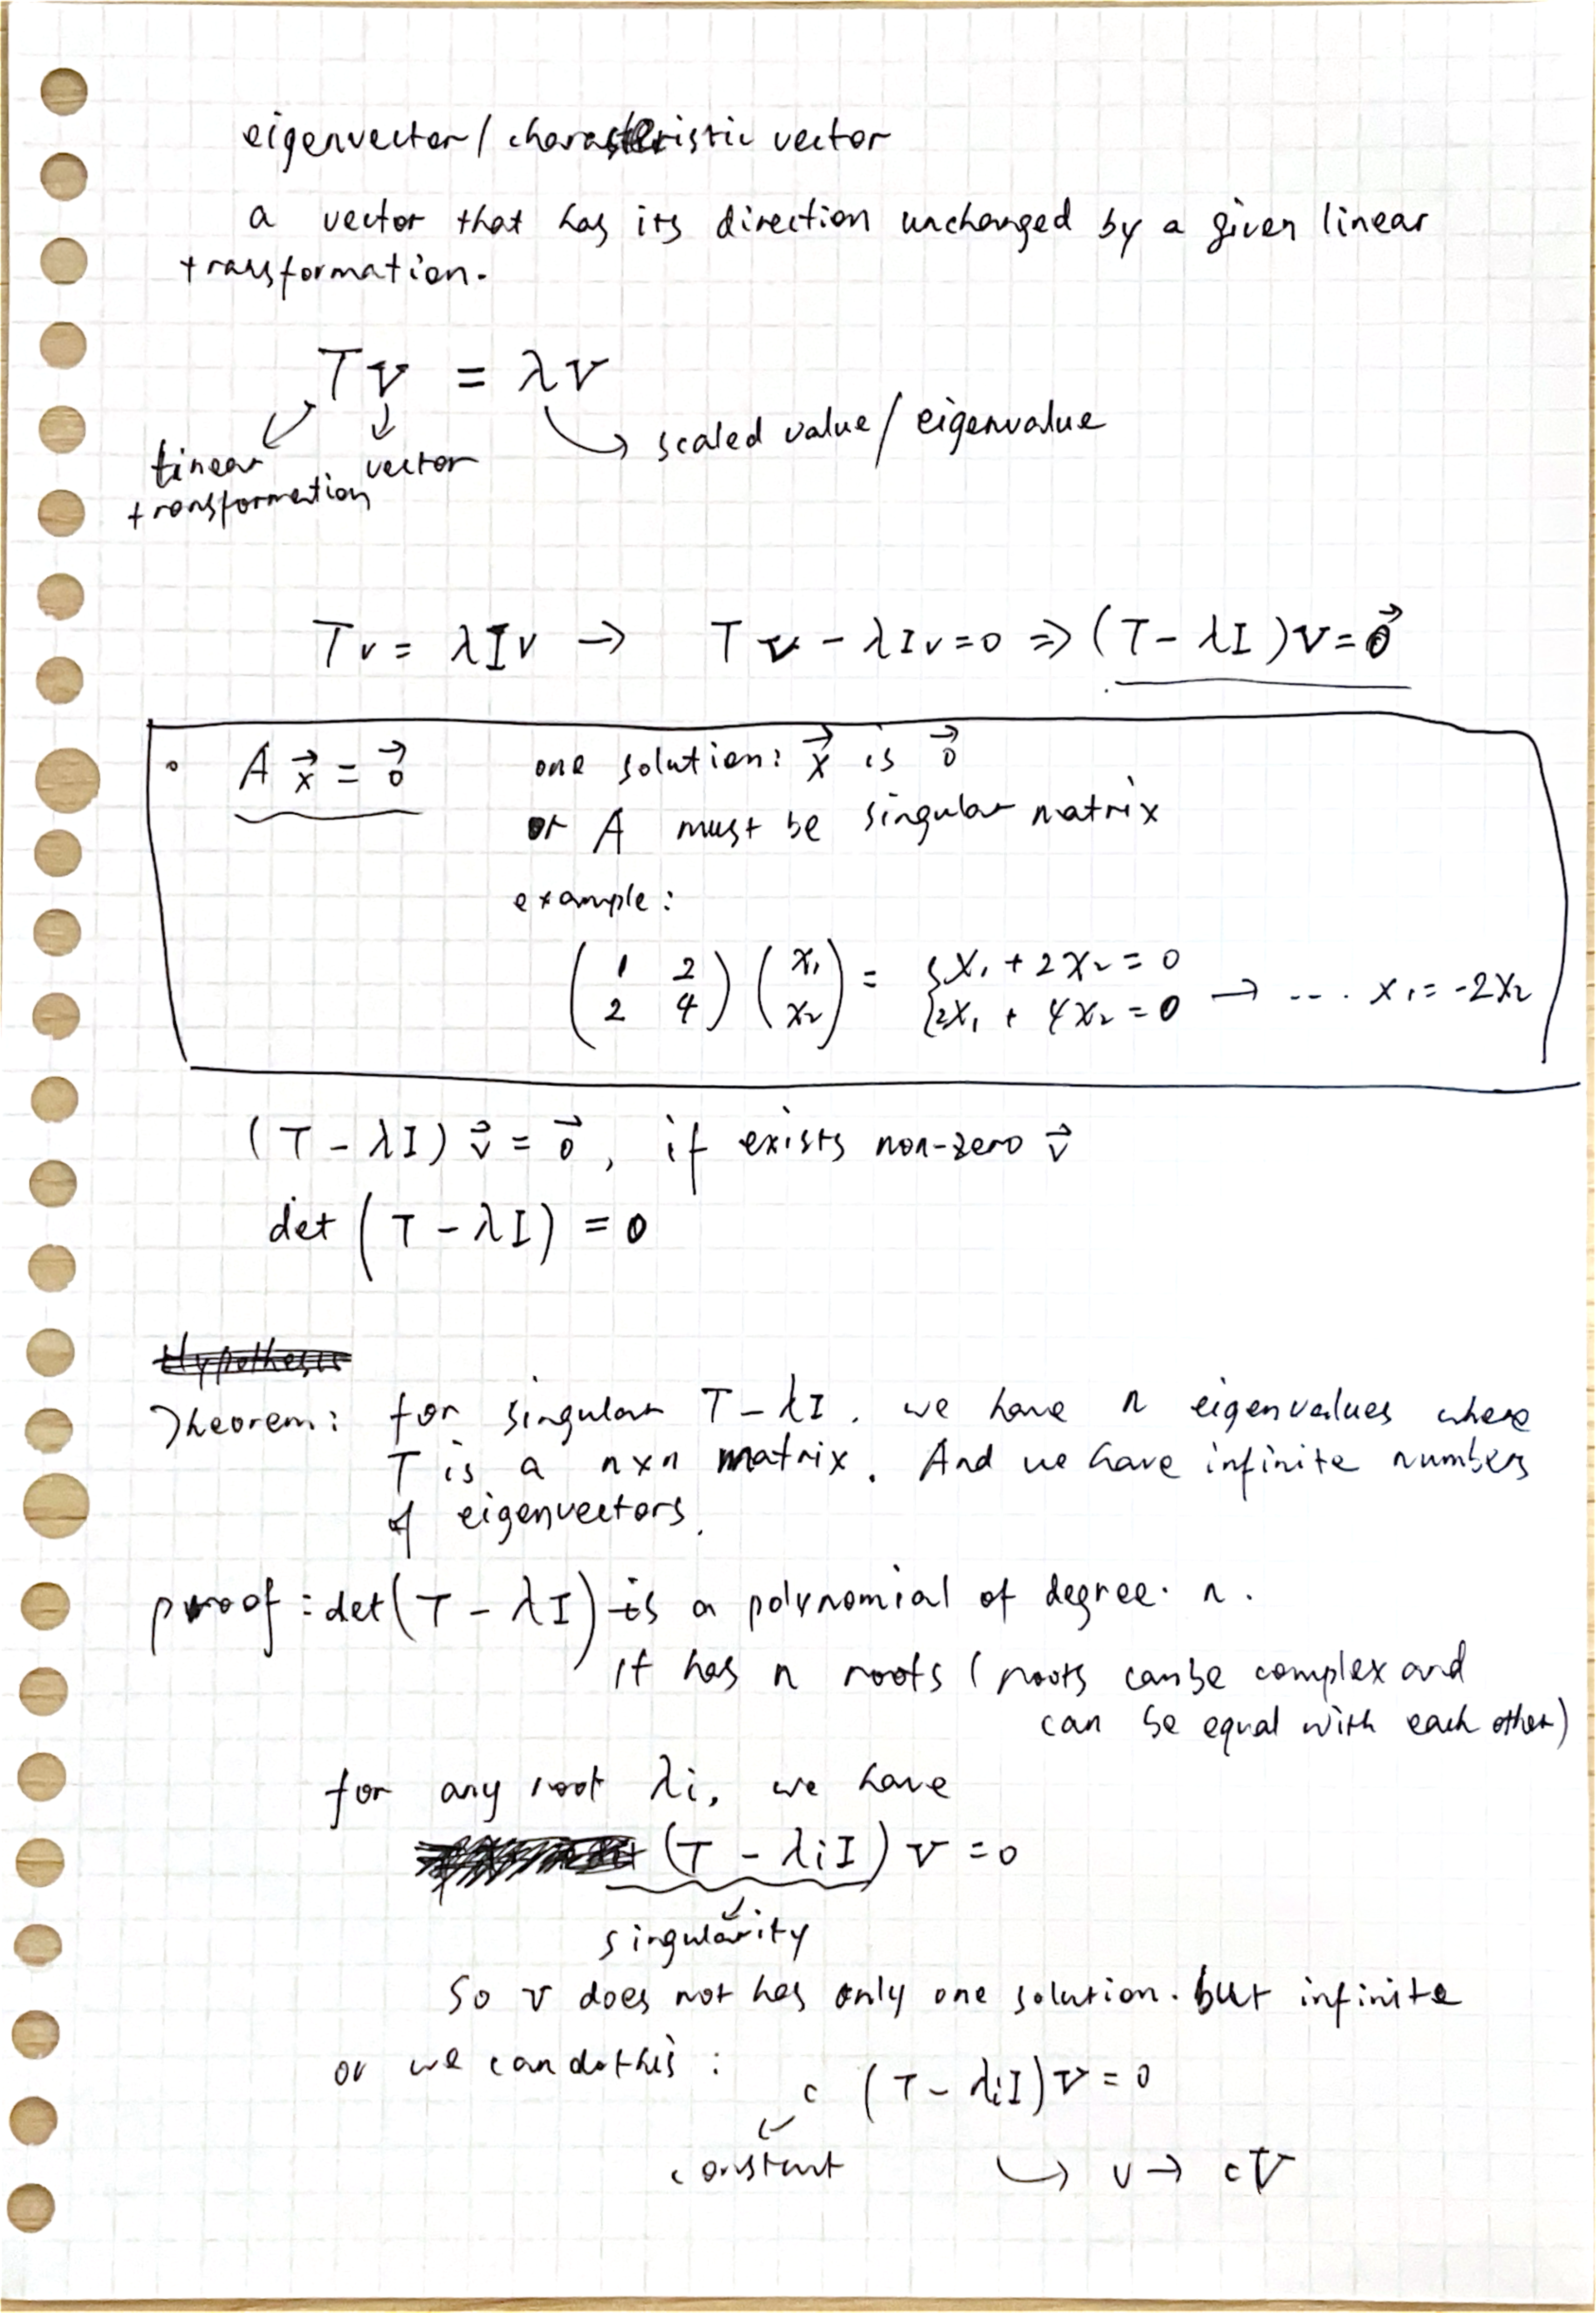
\includepdf[pages=-]{./Draft/eigenvalues.pdf}

\section{Diagonalization}

\begin{definition}[diagonalization]
   An $n  \times n$ matrix $A$ is diagonalizable if it is similar to a diagonal matrix, that is, if there exists an invertible $n \times n$ matrix $C$ and a diagonal matrix $D$ such that:

   $$A = C D C^{-1}$$
\end{definition}

\begin{eg}
    Any diagonal matrix is diagonalizable:  $D = IDI^{-1}$    
\end{eg}

\begin{theorem}[Diagonal Theorem]
    An $n \times n$ matrix A is diagonalizable if and only if $A$ has n linearly independent eigenvectors.

    In this case, $A = CDC^{-1}$ for:

    \[
    C = \begin{pmatrix}
        | & | &  & | \\
        v_1 & v_2 & \cdots & v_n \\
        | & | &  & | 
        \end{pmatrix},
        \qquad
    D = \begin{pmatrix}
        \lambda_1 & 0 & \cdots & 0  \\  
        0 & \lambda_2 & \cdots & 0 \\
        \vdots & \vdots & \ddots & \vdots \\
        0 & 0 & \cdots & \lambda_n 
    \end{pmatrix} 
    \]

    where $v_1, v_2, \dots v_n$  are linearly independent eigenvectors, and $\lambda_1, \lambda_2, \dots \lambda_n$ are the corresponding eignvalues, in the same order.
\end{theorem}

\begin{proof}
   proof 1: If A has n linearly independent eigenvectors - A is diagonalizable     \newline
   (a). $C = (v_1, v_2, \dots, v_n)$ composed of eigenvectors of A is invertible \newline
   (b). 
   \begin{align*}
        AC & = A \begin{pmatrix}
                v_1 & v_2 & \cdots & v_n
                \end{pmatrix} \\
            & = \begin{pmatrix}
                Av_1 & Av_2 & \cdots & Av_n
                \end{pmatrix} \\
            & = \begin{pmatrix}
                \lambda_1v_1 & \lambda_2v_2 & \cdots & \lambda_nv_n
                \end{pmatrix} \\
            & = \begin{pmatrix}
                    v_1 & v_2 & \cdots & v_n
                \end{pmatrix}
                \begin{pmatrix}
                    \lambda_1 & 0 & \cdots & 0  \\  
                    0 & \lambda_2 & \cdots & 0 \\
                    \vdots & \vdots & \ddots & \vdots \\
                    0 & 0 & \cdots & \lambda_n 
                \end{pmatrix} \\
            & = CD
   \end{align*}
   that is, $ACC^{-1} = CDC^{-1} \rightarrow A = CDC^{-1}$

   proof 2: A is diagonalizable - A has n linearly independent eigenvectors \newline
   A is diagonalizable means we can have $A = CDC^{-1}$ where D is a diagonal matrix. Multiply 2 sides of the equation with C, we have AC = CD. We can observe that: \newline
   Left side:
   \begin{align*}
    AC & = A \begin{pmatrix}
                v_1 & v_2 & \cdots & v_n
             \end{pmatrix} \\
       & = \begin{pmatrix}
                Av_1 & Av_2 & \cdots & Av_n
            \end{pmatrix}
   \end{align*}

   Right side:
   \begin{align*}
   CD & =  \begin{pmatrix}
             v_1 & v_2 & \cdots & v_n
           \end{pmatrix}
           \begin{pmatrix}
             \lambda_1 & 0 & \cdots & 0  \\  
             0 & \lambda_2 & \cdots & 0 \\
             \vdots & \vdots & \ddots & \vdots \\
             0 & 0 & \cdots & \lambda_n 
           \end{pmatrix} \\
        & = \begin{pmatrix}
           \lambda_1 v_1 & \lambda_2 v_2 & \cdots & \lambda_n v_n 
        \end{pmatrix}
   \end{align*}

   Which means for any i we have $Av_i = \lambda_i v_i$, so $\lambda_i$ is the eigenvalue and $v_i$  is the eigenvector.
\end{proof}

The above proof has referenced \href{https://leimao.github.io/blog/Matrix-Diagonalization-Theorem/}{this blog article} and \href{https://textbooks.math.gatech.edu/ila/diagonalization.html}{this online textbook from Gatech}.

\section{Complex Eigenvalue}

Since the characteristic equation of an \(n \times n\) matrix involves a polynomial of degree n, the equation always has exactly n roots.  

\begin{note}
    The characteristic equation is \((A - \lambda I) \vec{x}  = 0\) equation.

    N roots is guaranteed by fundamental theorem of algebra, we don't go any deeper here.
\end{note}

\begin{definition}[Complex Eigenvalue and Eigenvector]
    A complex scalar \(\lambda\)  satisfies \(det(A - \lambda I) = 0\) if and only if there is a nonzero vector x in \(\C^n\) such that \(Ax = \lambda x\), we call \(\lambda\) a \textbf{(complex) eigenvalue} and x a \textbf{(complex) eigenvector} corresponding to \(\lambda\)     
\end{definition}

\begin{eg}
    If \(A = \begin{bmatrix}
        0 &  -1 \\
        1 &  0 \\
    \end{bmatrix}\), then the linear transformation \(x \mapsto Ax\) on \(R^2\) rotates the plane counterclockwise through a quarter-turn. 

    Obviously, no nonzero vector is mapped into a multiple of itself, so A has no eigenvectoers in \(R^2\), and hence no real eigenvalues. 

    The characteristic equation of A is:
    \[
        \lambda^2 + 1 = 0
    \]

    The only 2 roots are complex \(\lambda = i\) and \(\lambda = -i\). If we permit A to act on \(\C^2\), then:
    \[
       \begin{bmatrix}
        0 &  -1 \\
        1 &  0 \\
       \end{bmatrix} 
       \begin{bmatrix}
         1 \\
         -i \\
       \end{bmatrix} 
        =
       \begin{bmatrix}
         i \\
         1 \\
       \end{bmatrix}
        =  
        i \begin{bmatrix}
             1 \\
             -i \\
        \end{bmatrix} \\
       \begin{bmatrix}
        0 &  -1 \\
        1 &  0 \\
       \end{bmatrix} 
       \begin{bmatrix}
         1 \\
         i \\
       \end{bmatrix} 
        =
       \begin{bmatrix}
         -i \\
         1 \\
       \end{bmatrix}
        =  
        -i \begin{bmatrix}
             1 \\
             i \\
        \end{bmatrix}
    \]   

    Then the eigenvectors are \(\begin{bmatrix}
         1 \\
         -i \\
    \end{bmatrix}\) and \(\begin{bmatrix}
         1 \\
         i \\
    \end{bmatrix}\)
\end{eg}

\subsection{Real and Imaginary Parts of Vectors}

\begin{eg}
    If \(x = \begin{bmatrix}
         3 - i \\
         i \\
         2 + 5i \\
    \end{bmatrix} =
    \begin{bmatrix}
         3 \\
         0 \\
         2 \\
    \end{bmatrix} + 
    i \begin{bmatrix}
         -1 \\
         1 \\
         5 \\
    \end{bmatrix}\), then we have \textbf{real part} \(x = \begin{bmatrix}
         3 \\
         0 \\
         2 \\
    \end{bmatrix} \), and \textbf{imaginary part} \(x = \begin{bmatrix}
         -1 \\
         1 \\
         5 \\
    \end{bmatrix}\), and  \(\overline{x}  = \begin{bmatrix}
         3 \\
         0 \\
         2 \\
    \end{bmatrix} - i \begin{bmatrix}
         -1 \\
         1 \\
         5 \\
    \end{bmatrix} = \begin{bmatrix}
         3 + i \\
         -i \\
         2 - 5i \\
    \end{bmatrix}\) in which entries are the complex conjugates of the entries in x. 
\end{eg}


\subsection{Eigenvalues and Eigenvectors of a Real Matrix That Acts on $C^n$}
%TODO. on page 300 of the book


\subsection{Problems}

\begin{problem}[Book Chapter 5.5 excercise 22]

\end{problem}

\begin{problem}[Book Chapter 5.5 excercise 23]

\end{problem}

\begin{problem}[Book Chapter 5.5 excercise 24]

\end{problem}